\subsubsection{Giới thiệu}
Bộ não con người và máy tính từ bản chất đã phù hợp với các loại công việc khác nhau. Ví dụ, việc tính căn bậc ba của một số lớn rất dễ dàng đối với máy tính, nhưng với con người thì vô cùng khó khăn. Trong khi đó, việc nhận diện các đối tượng trong một hình ảnh là một việc đơn giản đối với con người, nhưng lại rất khó khăn để con người có thể thực hiện một thuật toán tự động. Chỉ trong những năm gần đây, học sâu mới đã cho thấy độ chính xác trong một số công việc vượt qua cả của con người. Trên thực tế, các kết quả gần đây từ các thuật toán học sâu vượt qua con người trong việc nhận diện hình ảnh (chỉ trong một số trường hợp cụ thể), điều mà cách đây 20 năm được đánh giá là bất khả thi bởi các chuyên gia thị giác máy tính.\cite{Aggarwal2023}

Nhiều mạng thần kinh sinh học \textit{(biological neural networks)} đã cho thấy hiệu suất tính toán, nhận dạng một cách vượt trội dựa vào các kết nối thần kinh. Điều này cho thấy rằng mạng thần kinh sinh học đạt được hiệu suất ấy nhờ vào những kết nối đủ sâu, rộng và phức tạp. Thật không may là các mạng thần kinh sinh học được kết nối theo cách mà chúng ta chưa hiểu rõ. Trong những trường hợp ít ỏi mà chúng ta hiểu về cấu trúc mạng thần kinh sinh học, chúng ta đã áp dụng, tạo ra và phát triển mạng thần kinh nhân tạo dựa trên những hiểu biết đó. Một ví dụ điển hình về loại kiến trúc này là việc sử dụng mạng thần kinh tích chập \textit{(convolutional neural network)} cho việc nhận diện hình ảnh. Kiến trúc này đã được truyền cảm hứng từ các thí nghiệm của Hubel và Wiesel vào năm 1959 về tổ chức của các tế bào thần kinh trong vỏ não thị giác của mèo. Tiền đề cho mạng thần kinh tích chập là mạng thần kinh neocognitron, một mạng thần kinh được phát triển dựa trên thí nghiệm này.\cite{Aggarwal2023}

Cấu trúc kết nối tế bào thần kinh của con người đã tiến hóa qua hàng triệu năm để tối ưu hóa hiệu suất tính toán cho việc tồn tại. Và sự tồn tại này thì liên kết chặt chẽ với cảm giác và trực giác của con người theo một cách mà máy móc không thể giả lập lại được. Sinh lý học thần kinh là một lĩnh vực còn rất non trẻ và chúng ta chỉ mới hiểu biết rất ít về cách hoạt động thực sự của não bộ. Và khi lĩnh vực này phát triển mạnh sẽ mang đến những thành tựu khác được áp dụng khoa học máy tính, và ta có thể mong chờ rằng những thành tựu ấy sẽ thành công rực rỡ như sự thành công của mạng thần kinh tích chập.\cite{Aggarwal2023}

Một phần lớn thành tựu gần đây của các mạng thần kinh nhân tạo là do sự ra đời của dữ liệu lớn \textit{(big data)} cùng sức mạnh tính toán của máy tính hiện đại đã vượt qua giới hạn của các thuật toán học máy truyền thống, các thuật toán mà không thể tận dụng đầy đủ sức mạnh tính toán hiện nay. Đôi khi, các thuật toán học máy truyền thống lại tốt hơn khi mà các tập dữ liệu nhỏ hơn, các thuật toán này lại dễ dàng hơn trong giải thích mô hình, và xu hướng tạo ra những đặc trưng có thể giải thích bằng sự hiểu biết trong lĩnh vực đó. Với dữ liệu không đủ lớn, ta sử dụng nhiều mô hình truyền thống và chọn ra mô hình tốt nhất thường sẽ mang lại kết quả tốt hơn so với việc trực tiếp sử dụng mạng thần kinh nhân tạo. Điều này là một trong những lý do tại sao tiềm năng của mạng thần kinh nhân tạo không được đánh giá cao khi nó mới được phát triển.

Thời đại dữ liệu lớn đã được kích hoạt bởi sự tiến bộ trong công nghệ thu thập dữ liệu. Gần như mọi việc chúng ta làm ngày nay, bao gồm việc mua một món hàng, sử dụng điện thoại, hoặc nhấp chuột vào một trang web, đều được thu thập và lưu trữ ở một nơi nào đó. Hơn nữa, sự phát triển của bộ xử lý đồ hoạ \textit{(Graphics Processor Units – GPU)} đã cho phép xử lý hàng trăm triệu các phép tính mỗi giây và nhân các ma trận với hàng triệu phần tử, điều mà bộ xử lý trung tâm \textit{(CPU)} không thể đạt được. Những tiến bộ này cho phép chúng ta sử dụng các thuật toán học sâu \textit{(deep learning)} được nghiên cứu từ hai thập kỷ trước chỉ với sự tinh chỉnh không đáng kể. Trong quá khứ, nếu cần một tháng để kiểm thử một thuật toán, thì tối đa ta chỉ có thể kiểm thử mười hai biến thể trong một năm. Điều này từng hạn chế việc kiểm thử chuyên sâu để điều chỉnh nghiệm trong các thuật toán mạng thần kinh nhân tạo. Đặc biệt, các tiến bộ nhanh chóng liên quan đến ba trụ cột trong ngành là: dữ liệu, tính toán, và thử nghiệm đã mở ra một tương lai rộng mở của học sâu. Vào cuối thế kỷ này, người ta dự kiến rằng máy tính sẽ có khả năng huấn luyện mạng thần kinh nhân tạo với số lượng tế bào thần kinh tương đương với não bộ con người.\cite{Aggarwal2023}
\begin{figure}[htb]
    \centering
    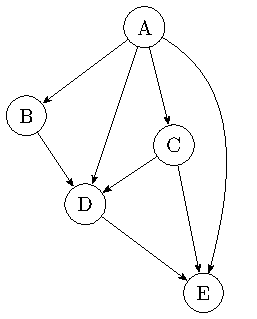
\includegraphics[width=0.25\textwidth]{tikz_image/directed_acyclic_graph.pdf}
    \caption{Đồ thị không có chu trình}
    \label{figure:directed-acyclic-graph}
\end{figure}

Mạng thần kinh có dạng đồ thị không có chu trình \textit{(directed acyclic graph)} (Hình \ref{figure:directed-acyclic-graph}) bao gồm các cạnh và các nút. Các cạnh của mạng là các tham số. Các nút chứa một giá trị cố định (nếu là nút đầu vào) hoặc giá trị được tính toán từ các cặp nút - cạnh kết nối đến nó. Nên có thể xem mạng thần kinh chỉ là sự tính toán các hàm từ các nút đầu vào đến các nút đầu ra.

Trong mạng một lớp, một tập hợp các nút đầu vào được kết nối trực tiếp với một hoặc nhiều nút đầu ra. Trong mạng nhiều lớp, các nơron được sắp xếp thành nhiều lớp liên tiếp nhau, trong đó các lớp đầu vào và đầu ra được tách ra bởi một nhóm các lớp ẩn các nút.

\subsubsection{Mạng thần kinh nhân tạo một lớp - \textit{(Single-layer Neural Network - Perceptron)}}
Mạng thần kinh nhân tạo đơn giản nhất có một lớp được gọi là perceptron (Hình \ref{figure:single-layer-network}). Mạng này bao gồm một lớp đầu vào và một nút đầu ra. Ta ký hiệu đầu vào bằng vector $\mathbf{x}$ và đầu ra là một số $y$. Lớp đầu vào chứa $d$ nút nên có thể viết đầu vào là một vector $\mathbf{x} = [x_1\dots x_d]$.
\begin{figure}[htb]
    \centering
    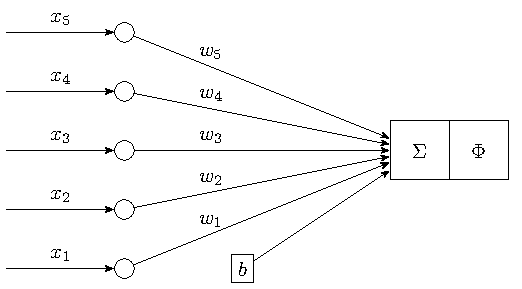
\includegraphics[width=0.5\textwidth]{tikz_image/perceptron.pdf}
    \caption{Cấu tạo mạng thần kinh nhân tạo đơn giản}
    \label{figure:single-layer-network}
\end{figure}

Để đơn giản ta quy định đầu ra $y$ là một biến nhị phân \textit{(binary)} $y\in\{-1,+1\}$. Lớp đầu vào là các nút được liên kết với các cạnh có trọng số $w_1,\dots,w_d$ ($\mathbf{w}=[w_1,\dots,w_d]$), tất cả các cạnh này được kết nối với một nút đầu ra duy nhất. Một hàm tuyến tính được hình thành từ đầu vào $\mathbf{x}$ và trọng số $\mathbf{w}$ là $\mathbf{w^\intercal x}=\sum^d_{i=1}w_ix_i$ sẽ tính giá trị đầu ra rồi đưa giá trị này vào hàm $\text(sign)(\cdot)$. Vậy nên giá trị dự đoán $\hat{y}$ là
\begin{align}
    \hat{y}=f(\mathbf{x})=\text(sign)(\mathbf{w^\intercal x})=\text(sign)(\sum^d_{i=1}w_ix_i)
\end{align}
Hàm sign chuyển đổi một giá trị thực thành $+1$ hoặc $-1$, nghĩa là bài toán perceptron trong ví dụ trên giống với bài toán phân loại nhị phân \textit{(binary classification)}. Ta chọn một hàm mất mát \textit{loss function} để đánh giá độ lệch giữa giá trị quan sát $y$ với giá trị dự đoán $\hat{y}$. Ban đầu hàm $f(\cdot)$ với trọng số $\mathbf{w}$ được tạo ngẫu nhiên. Với mỗi đầu vào $\mathbf{x}$, ta thay đổi trọng số $\mathbf{w}$ để giá trị đầu ra giống dữ liệu huấn luyện, làm hàm $f(\cdot)$ có độ chính xác cao hơn. Quá trình này lặp đi lặp lại để nhận được trọng số $\mathbf{w}$ tốt nhất, làm cho tổng mất mát trên toàn bộ dữ liệu huấn luyện là thấp nhất được gọi là quá trình học \textit{(learning)}.

Thời điểm sơ khai khi lĩnh vực học máy chưa phát triển, hàm mất mát của thuật toán chưa được tối ưu hoá mà chỉ được xây dựng trên những kinh nghiệm một cách tự nhiên \textit{(heuristic)}. Với đầu vào là $\mathbf{x}$, giá trị dự đoán sẽ là $\hat{y}=f(\mathbf{x})=\text(sign)(\mathbf{w^\intercal x})$. Khi giá trị dự đoán $\hat{y}$ khác giá trị quan sát $\hat{y}\neq y\in\{-1,+1\}$ thì trọng số $\mathbf{w}$ sẽ được cập nhật dựa trên $(y-\hat{y})$
\begin{align}
    \mathbf{w}\Leftarrow\mathbf{w}+\alpha(y-\hat{y})\mathbf{x}
\end{align}
Với số $\alpha$ được gọi là tỉ lệ học \textit{(learning rate)}. Thuật toán perceptron bây giờ là quá trình duyệt qua toàn bộ dữ liệu một cách ngẫu nhiên, lặp đi lặp lại với hữu hạn lần (mỗi chu kỳ lặp được gọi là 1 \textit{epoch}). Mỗi lần duyệt qua một điểm sẽ cập nhật lại trọng số $\mathbf{w}$, sao cho khi học xong toàn bộ tập dữ liệu sẽ cho ra một mô hình \textit{(model)} dự báo đúng trên toàn bộ tập dữ liệu, khi đó ta gọi thuật toán đạt được sự hội tụ \textit{(convergence)}. Giá trị của $(y-\hat{y})$ luôn là $2y$ khi $\hat{y}\neq y$, nên ta có thể viết lại
\begin{align}
    \mathbf{w}\Leftarrow\mathbf{w}+2\alpha y\mathbf{x}\sim\mathbf{w}+\alpha y\mathbf{x}
\end{align}

Bài toán perceptron cũng được coi là một mô hình tuyến tính \textit{(linear model)}, bởi vì phương trình $\mathbf{w^\intercal x}=0$ định nghĩa một siêu phẳng \textit{(hyperplane)}, với $\mathbf{w}=[w_1,\dots,w_d]$ là một vector $d$ chiều trực giao \textit{(perpendicular)} với siêu phẳng. Siêu phẳng này chia không gian thành hai nửa, các điểm dữ liệu hoặc thuộc về nửa dương \textit{(positive)} khi $\mathbf{w^\intercal x}>0$ hoặc thuộc về nửa âm \textit{(negative)} khi $\mathbf{w^\intercal x}<0$. Mô hình này chạy tốt khi tập dữ liệu là phân biệt tuyến tính \textit{(linearly separable)} (Hình \ref{figure:linearly-separable}), nghĩa là có tồn tại một siêu phẳng chia các điểm dữ liệu thành hai phần, mỗi phần thuộc về một class khác nhau. Thuật toán này đã được Rosenblatt chứng minh là hội tụ khi và chỉ khi tập dữ liệu là phân biệt tuyến tính.\cite{Aggarwal2023}
\begin{figure}[htbp]
    \centering
    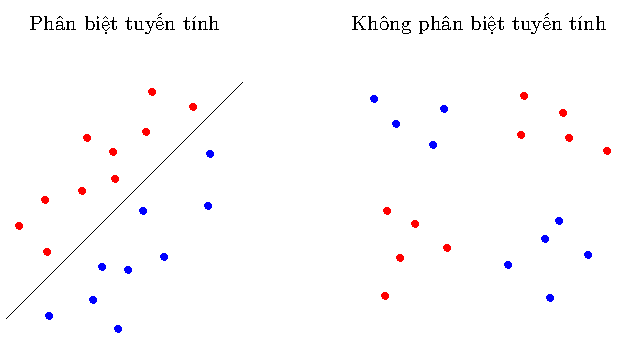
\includegraphics[width=0.6\textwidth]{tikz_image/linearly_separable.pdf}
    \caption{Phân biệt tuyến tính}
    \label{figure:linearly-separable}
\end{figure}

Đối với tập dữ liệu có phân phối nhị phân \textit{(binary class distribution)} bị mất cân bằng \textit{(imbalanced)}, như trong bài toán phân loại nhị phân là trường hợp trung bình của các điểm có nhãn $\{-1, +1\}$ khác $0$
\begin{align}
    \underbrace{\sum_i y_i}_{\neq 0}\neq\underbrace{\sum_i\hat{y_i}}_{=0}=\sum_i\text(sign)(\mathbf{w}^\intercal\mathbf{x_i})
\end{align}
Khi tập dữ liệu mất cân bằng càng nhiều, thuật toán perceptron càng mất chính xác. Để khắc phục điều này, ta cộng thêm một lượng nhỏ b (\textit{bias}) vô giá trị dự đoán để làm cho giá trị này bị mất cân bằng
\begin{align}
    \hat{y}=\text(sign)(\mathbf{w^\intercal x}+b)=\text(sign)(\sum^d_{i=1}w_ix_i+b)
\end{align}
Và ta sẽ điều chỉnh $b$ để kết quả dự báo mất cân bằng giống với cách mà giá trị quan sát mất cân bằng.

\subsubsection{Hàm kích hoạt - \textit{(Activation Function)}}
Hàm kích hoạt được định nghĩa là một giá trị dự đoán $\Phi$ có dạng
\begin{align}
    \hat{y}=\Phi(\mathbf{w}^\intercal\mathbf{x})
\end{align}

Ta chia một nút bất kì (khác nút đầu vô) thành 2 giai đoạn, giá trị của nút trước khi áp dụng hàm kích hoạt gọi là \textit{pre-activation value}, ngược lại là \textit{post-activation value} (hình \ref{figure:pre-post-activation-value}).
\begin{figure}[htb]
    \centering
    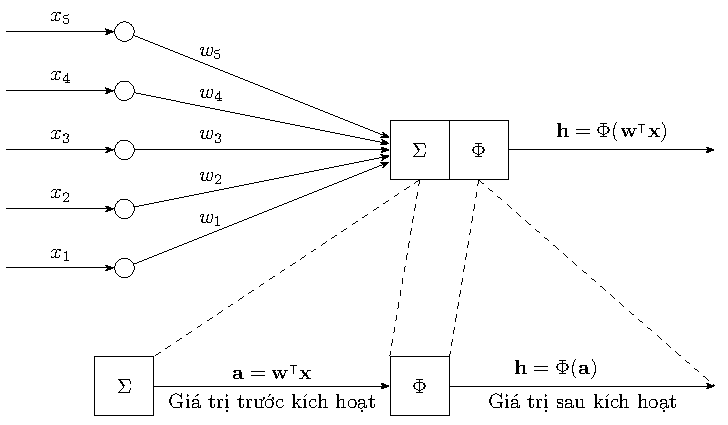
\includegraphics[width=0.6\textwidth]{tikz_image/pre_post_activation_value.pdf}
    \caption{Giá trị trước khi kích hoạt và giá trị sau khi kích hoạt}
    \label{figure:pre-post-activation-value}
\end{figure}

Hàm kích hoạt thường thấy nhất là hàm tuyến tính. Hàm tuyến tính thường được sử dụng ở các nút đầu ra vì thường chúng ta mong muốn đầu ra là một số thực nào đó.
\begin{align}
    \Phi(v)=v
\end{align}
Hàm kích hoạt phi tuyến được sử dụng trong những ngày đầu phát triển của mạng thần kinh nhân tạo là hàm sign, hàm sigmoid, hàm tanh (hình \ref{figure:activation-funtion-1}).
\begin{align}
    \Phi(v) & =\text(sign)(v)                   & \text{[hàm sign]}    \\
    \Phi(v) & =\dfrac{1}{1+e^{-v}}        & \text{[hàm sigmoid]} \\
    \Phi(v) & =\dfrac{e^{2v}-1}{e^{2v}+1} & \text{[hàm tanh]}
\end{align}
\begin{figure}[htb]
    \centering
    \begin{subfigure}[b]{0.25\textwidth}
        \centering
        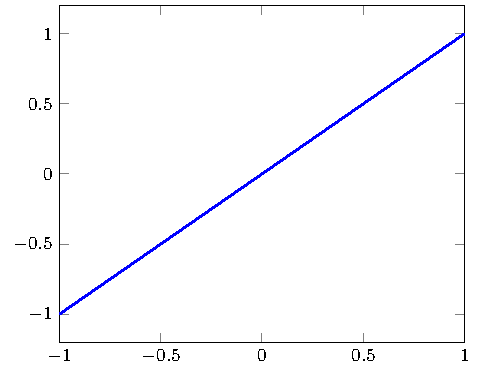
\includegraphics[width=\textwidth]{tikz_image/identity.pdf}
        \caption{Hàm tuyến tính}
    \end{subfigure}%
    \begin{subfigure}[b]{0.25\textwidth}
        \centering
        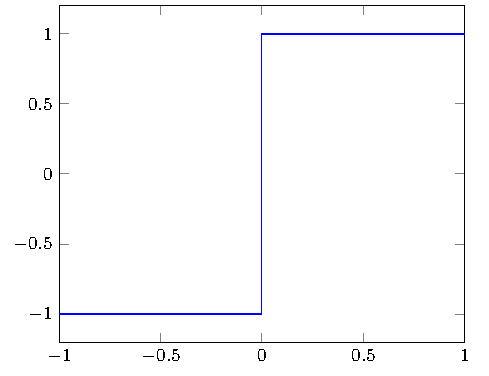
\includegraphics[width=\textwidth]{tikz_image/sign.pdf}
        \caption{Hàm sign}
    \end{subfigure}%
    \begin{subfigure}[b]{0.25\textwidth}
        \centering
        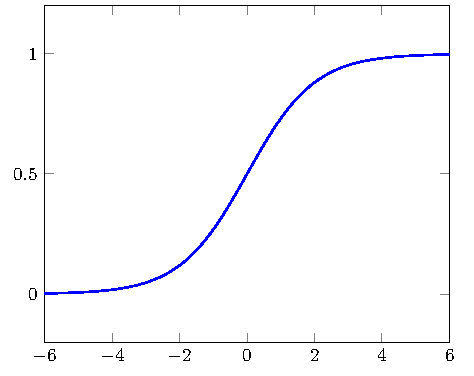
\includegraphics[width=\textwidth]{tikz_image/sigmoid.pdf}
        \caption{Hàm sigmoid}
    \end{subfigure}%
    \begin{subfigure}[b]{0.25\textwidth}
        \centering
        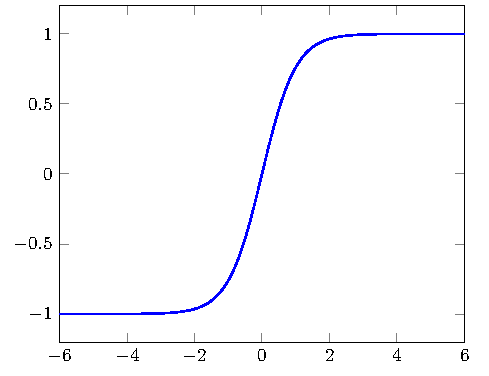
\includegraphics[width=\textwidth]{tikz_image/tanh.pdf}
        \caption{Hàm tanh}
    \end{subfigure}%
    \caption{Đồ thị các hàm kích hoạt thông dụng}
    \label{figure:activation-funtion-1}
\end{figure}
\begin{figure}[htb]
    \centering
    \begin{subfigure}[b]{0.4\textwidth}
        \centering
        \includegraphics[width=\textwidth]{tikz_image/reLU.pdf}
        \caption{Hàm ReLU}
    \end{subfigure}%
    \begin{subfigure}[b]{0.4\textwidth}
        \centering
        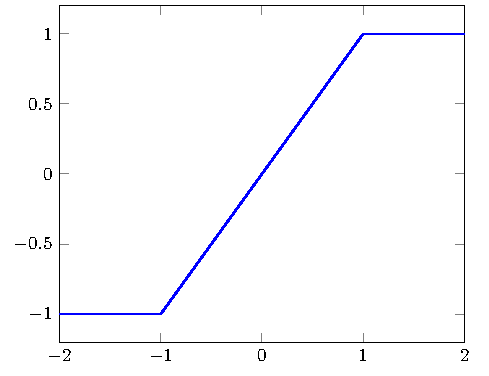
\includegraphics[width=\textwidth]{tikz_image/hardtanh.pdf}
        \caption{Hàm hardtanh}
    \end{subfigure}%
    \caption{Đồ thị các hàm kích hoạt tuyến tính từng phần}
    \label{figure:activation-function-2}
\end{figure}
Hàm sigmoid cho ra giá trị từ $(0,1)$ sẽ phù hợp khi dùng cho đầu ra có dạng xác suất. Đồ thị hàm tanh khá giống hàm sigmoid nhưng khác ở điểm nó có đầu ra từ $[-1,1]$, và thường được ưu tiên hơn hàm sigmoid vì nó cho cả giá trị âm. Điểm yếu của các hàm phi tuyến là chúng quá dễ đạt đến giá trị bão hoà (giá trị sẽ không thay đổi nhiều trong khoảng lân cận) khi mà giá trị đầu vào lớn đến một mức nào đó, ví dụ hàm sigmoid khi $x>6$ thì giá trị $y_{x>6}$ sẽ không khác nhau nhiều. Nhưng ngược lại hàm phi tuyến lại giúp ta chuẩn hoá giá trị đầu ra về một khoảng xác định (ví dụ đối với hàm sigmoid là $(0,1)$).

Trong những năm gần đây, hàm kích hoạt tuyến tính từng phần \textit{(piecewise linear activation functions)} được ưu tiên sử dụng hơn, vì nó không có điểm bão hoà, và các hàm này sẽ được tính nhanh hơn trong máy tính, giúp tối ưu đáng kể hiệu suất. Ví dụ là hàm ReLU và hàm hardtanh (hình \ref{figure:activation-function-2}).
\begin{align}
    \Phi(v) & =\max(v,0)          & \text{[hàm Rectified Linear Unit (ReLU)]} \\
    \Phi(v) & =\max(\min(v,1),-1) & \text{[hàm hardtanh]}
\end{align}

\subsubsection{Hàm kích hoạt Softmax - \textit{(Softmax Activation Function)}}
Hàm kích hoạt softmax là một hàm đặc biệt vì nó thường được sử dụng trong lớp đầu ra để ánh xạ $k$ giá trị thực thành $k$ xác suất của các sự kiện rời rạc, và tổng xác suất của các sự kiện này là $1$. Ví dụ, trong bài toán phân loại sản phẩm vào $k$ lớp khác nhau, trong đó mỗi sản phẩm cần được đánh nhãn là một trong $k$ lớp đó.
\begin{align}
    \Phi(v_i)=\dfrac{\exp(v_i)}{\sum^k_{j=1}\exp(v_j)}\quad\forall i\in\{1,\dots,k\}
\end{align}

Hình \ref{figure:softmax-layer} là ví dụ của hàm softmax với các giá trị đầu ra là $v_1, v_2, v_3$, và lớp softmax \textit{(softmax layer)} biến đổi các giá trị này thành xác suất của $3$ lớp khác nhau. Đối với lớp softmax, các cạnh nối với lớp này sẽ có hệ số là $1$.
\begin{figure}[htb]
    \centering
    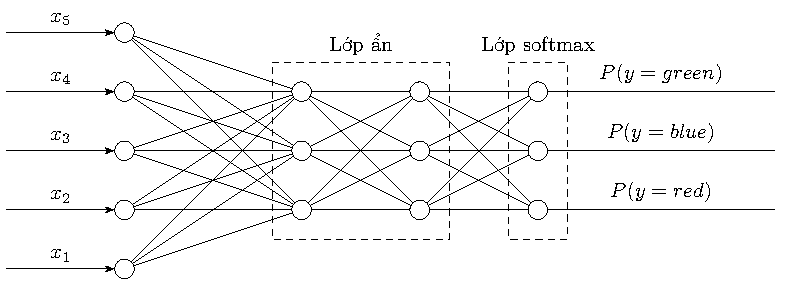
\includegraphics[width=0.7\textwidth]{tikz_image/softmax_layer.pdf}
    \caption{Mạng thần kinh nhân tạo với lớp softmax làm lớp đầu ra}
    \label{figure:softmax-layer}
\end{figure}

\subsubsection{Hàm mất mát - \textit{(Lost Function)}}
Thông thường, hàm mất mát được định nghĩa phụ thuộc vào đầu ra của mô hình và dữ liệu hiện có. Các hàm mất mát thường dùng được phân thành 2 loại \cite{ciampiconi2023surveytaxonomylossfunctions}:
\begin{itemize}
    \item Hàm mất mát dùng cho hồi quy \textit{(Regression Losses)}
          \begin{enumerate}
              \item Mean bias error loss
                    \begin{align}
                        L_{MBE}=\dfrac{1}{N}\sum_{i=1}^N\left(y_i-\hat y_i\right)
                    \end{align}
              \item Mean absolute error loss - L1 loss
                    \begin{align}
                        L_{MAE}=\dfrac{1}{N}\sum_{i=1}^N\left|y_i-\hat y_i\right|
                    \end{align}
              \item Mean squared error loss - L2 loss
                    \begin{align}
                        L_{MAE}=\dfrac{1}{N}\sum_{i=1}^N\left(y_i-\hat y_i\right)^2
                    \end{align}
          \end{enumerate}
          và một số hàm khác như Root mean squared error loss, Huber loss, v.v..
    \item Hàm mất mát dùng cho phân loại \textit{(Classification Losses)}
          \begin{enumerate}
              \item Zero-One loss
                    \begin{align}
                        L_\text{ZeroOne}(y,\hat y)=
                        \begin{cases}
                            1\quad\text{if }y\cdot\hat y<0 \\
                            0\quad\text{otherwise}
                        \end{cases}
                    \end{align}
              \item Hinge loss
                    \begin{align}
                        L_\text{Hinge}(y,\hat y)=\max(0,1-(y\cdot\hat y))
                    \end{align}
              \item Cross Entropy loss
                    \begin{align}
                        L_\text{CrossEntropy}=-\sum_{i=1}^N y_i\log(\hat y_i)
                    \end{align}
          \end{enumerate}
          và một số hàm khác như Ramp loss, Cosine Similarity loss, v.v..
\end{itemize}

\subsubsection{Mạng thần kinh nhân tạo nhiều lớp - \textit{(Multi-Layer Neural Networks)}}
Đối với mạng thần kinh nhân tạo một lớp thì ai cũng có thể thấy được toàn bộ quá trình tính toán, bởi vì nó chỉ gồm hai lớp là lớp đầu vào và lớp đầu ra. Nhưng đối với mạng thần kinh nhiều lớp có sự tồn tại của các lớp ẩn, thì quá trình tính toán giữa các lớp ẩn này là hoàn toàn không nhìn thấy được.
\begin{figure}[htbp]
    \centering
    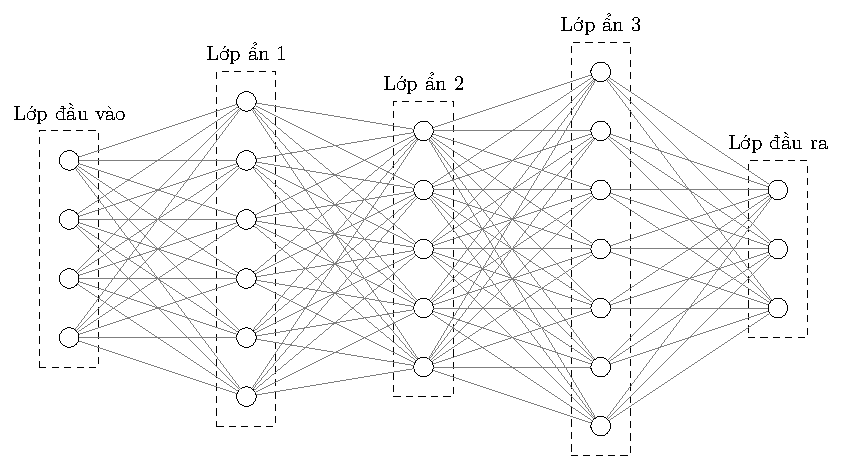
\includegraphics[width=0.8\textwidth]{tikz_image/multi_layer_neural_network.pdf}
    \caption{Mạng thần kinh nhiều lớp}
    \label{figure:multi-layer-nn}
\end{figure}

Kiến trúc cụ thể của mạng thần kinh nhiều lớp được gọi là mạng thần kinh truyền thẳng \textit{(feed-forward networks)}. Trong mạng thần kinh truyền thẳng, các lớp liên tiếp truyền dữ liệu cho nhau theo hướng từ lớp đầu vào đến lớp đầu ra, tất cả các nút trong một lớp được kết nối với các nút của lớp tiếp theo.

Ta có thể biểu diễn sự kết nối giữa các lớp này bằng phép nhân ma trận. Nếu mạng thần kinh có $k$ lớp ẩn, trong mỗi lớp có $p_1\dots p_k$ nốt, thì vector kết quả $\mathbf h_1\dots\mathbf h_k$ ở mỗi lớp ẩn này sẽ có số chiều \textit{(dimension)} lần lượt là $p_1\dots p_k$. Xét lớp đầu vào và lớp ẩn đầu tiên, nếu $d$ là số nốt của lớp đầu vào, $W_1$ là ma trận chứa các trọng số $w_i$ từ lớp đầu vào đến lớp ẩn đầu tiên, thì ma trận này có kích thước là $p_1\times d$. Tương tự nếu ta xét kết nối giữa lớp ẩn $r$ và lớp ẩn $r+1$, thì ma trận trọng số $W_{r+1}$ sẽ có kích thước là $p_{r+1}\times p_r$. Nếu lớp đầu ra của mạng có $o$ nốt thì ma trận trọng số $W_{k+1}$ sẽ có kích thước $o\times p_k$. Nếu gọi $\Phi$ là hàm kích hoạt thì
\begin{align}
    \label{equation:matrix-form}
    \mathbf h_1     & =\Phi(W_1\mathbf x)       & \text{[Từ lớp đầu vào đến lớp ẩn đầu tiên]} \\
    \mathbf h_{p+1} & =\Phi(W_{p+1}\mathbf h_p) & \text{[Giữa các lớp ẩn]}                    \\
    \mathbf o       & =\Phi(W_{k+1}\mathbf h_k) & \text{[Từ lớp ẩn cuối cùng đến lớp đầu ra]}
\end{align}
\begin{figure}[htbp]
    \centering
    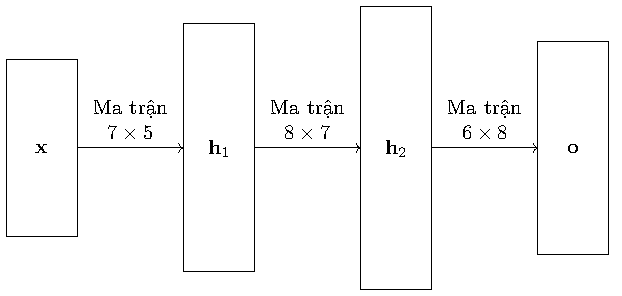
\includegraphics[width=0.6\textwidth]{tikz_image/multi_layer_matrix.pdf}
    \caption{Mạng thần kinh nhiều lớp với cách biểu diễn dưới dạng ma trận}
    \label{figure:multi-layer-matrix}
\end{figure}

Nếu ta sử dụng hàm kích hoạt tuyến tính ($\Phi(x)=x$) cho toàn bộ nút trong mạng, thì đầu ra $\mathbf o$ có thể được viết lại thành
\begin{align}
    \mathbf o & =W_{k+1}\mathbf h_k                                 \nonumber \\
              & =W_{k+1}W_k\mathbf h_{k-1}                          \nonumber \\
              & \quad\dots                                          \nonumber \\
              & =\underbrace{W_{k+1}W_k\dots W_1}_{W_{xo}}\mathbf x
\end{align}
Nghĩa là dù mô hình mạng của ta có nhiều lớp, nhưng mô hình cuối cùng cũng chỉ tương đương với mô hình mạng một lớp tuyến tính \textit{(single-layer linear network)}, điều này làm mất đi điểm mạnh của mô hình mạng nhiều lớp.

Ngoài cách biểu diễn bằng phép nhân ma trận, ta có thể biểu mạng thần kinh nhân tạo bằng đồ thị tính toán \textit{(computational graph)} (Hình \ref{figure:computational-graph}).
\begin{figure}[htbp]
    \centering
    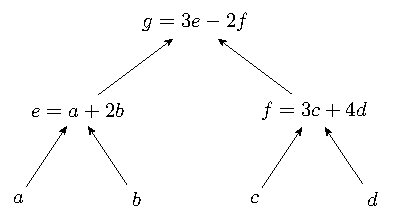
\includegraphics[width=0.4\textwidth]{tikz_image/computational_graph.pdf}
    \caption{Đồ thị tính toán}
    \label{figure:computational-graph}
\end{figure}

Nếu ta định nghĩa $g(\cdot)$ là hàm tính giá trị của một nốt ở lớp $m$, $f(\cdot)$ là hàm tính giá trị nốt ở lớp $m+1$, thì  giá trị của nốt ở lớp $m$ đó sẽ có dạng $f(g_1,\dots,g_k)$, với tham số của các hàm chính là trọng số của các cạnh. Nghĩa là ta có thể xây dựng một hàm số tổng quát kết nối từ lớp đầu vào, thông qua tất cả các lớp ẩn, đến lớp đầu ra. Quá trình học máy bây giờ được rút gọn thành việc lựa chọn các tham số cho các hàm này sao cho giá trị thực sự và giá trị dự đoán trùng nhau. Nhưng để tìm được một hàm tổng quát (\textit{closed-form}) ngắn gọn để biểu diễn cả mạng thần kinh nhân tạo là điều gần như không thể, bởi vì đây là các hàm lồng vô nhau nên khi càng có nhiều lớp ẩn thì hàm tổng quát này càng phức tạp. Chính điều này dẫn đến việc ta không thể áp dụng thuật toán xuống dốc \textit{(gradient descent)} để tìm tham số tối ưu. Thuật toán lan truyền ngược \textit{(backpropagation algorithm)} được sinh ra để giải quyết vấn đề này.\cite{Aggarwal2023}

\subsubsection{Thuật toán lan truyền ngược - \textit{(Backpropagation Algorithm)}}
Như đã nói bên trên, khi biểu diễn mạng thần kinh nhân tạo dưới dạng đồ thị tính toán, để tính giá trị của một nút ta cần phải tính giá trị của tất cả các nút ở lớp trước đó. Ví dụ mạng thần kinh nhân tạo với mỗi lớp chỉ có duy nhất một nút, hàm để tính giá trị của nút ở lớp $m$ là $g(x)$, ở lớp $m+1$ là $f(x)$, nếu ta chọn $f(x)=g(x)$ là hàm sigmoid, thì giá trị của nút ở lớp $m+1$ là
\begin{align}
    f(g(x))=\dfrac{1}{1+\exp\left[-\dfrac{1}{1+\exp(-x)}\right]}
\end{align}
Nếu ta tiếp tục tăng số lớp lên, thì giá trị của nút ở lớp $m+n$ sẽ có dạng
\begin{align}
    f(\cdots z(x))=\dfrac{1}{1+\exp\left[-\dfrac{1}{1+\exp\left[-\cdots-\dfrac{1}{1+\exp(-x)}\right]}\right]}
    \label{equation:expansion-formula-nn}
\end{align}

Đối với các thuật toán học máy truyền thống, ta phải tìm hàm $\hat{y}=f(\mathbf{x},\mathbf{w})$, rồi ta chọn một hàm mất mát để đánh giá sai số giữa $\hat{y}$ và $y$. Hàm mất mát này sẽ có dạng $L=L(y,\hat{y})=L(y,\mathbf{x},\mathbf{w})$. Sau đó ta phải khai triển đại số và rút gọn $L$, rồi áp dụng thuật toán xuống đồi để tối ưu vector $\mathbf{w}$. Để đơn giản hoá, thay vì tính đạo hàm của hàm mất mát $L$, ta sẽ tính đạo hàm của $\hat{y}$, rồi từ đó suy ngược lại đạo hàm của $L(y,\hat{y})$. Đối với mạng thần kinh nhân tạo, việc tìm ra công thức rút gọn của $\hat{y}$ gần như là không thể vì nó thường là các hàm phi tuyến lồng vô nhau, nghĩa là công thức của hàm này sẽ rất dài và phức tạp (ví dụ trong hàm \ref{equation:expansion-formula-nn}) dẫn đến việc tính đạo hàm này sẽ trở nên khó khăn, và độ khó khăn sẽ tăng lên càng cao nếu như ta tăng số lượng lớp. Đây là vấn đề đầu tiên khi dùng phương pháp giải thuật toán học máy truyền thống để tối ưu mạng thần kinh nhân tạo.

Vấn đề thứ hai gặp phải là độ phức tạp sẽ tăng khi ta tăng số lượng nút trong lớp. Xét một mạng thần kinh có $n$ lớp, mỗi lớp có 2 nút, biểu diễn đồ thị tính toán ở hình \ref{figure:computational-graph-of-n-layer-2-node-nn}.
\begin{figure}[htb]
    \centering
    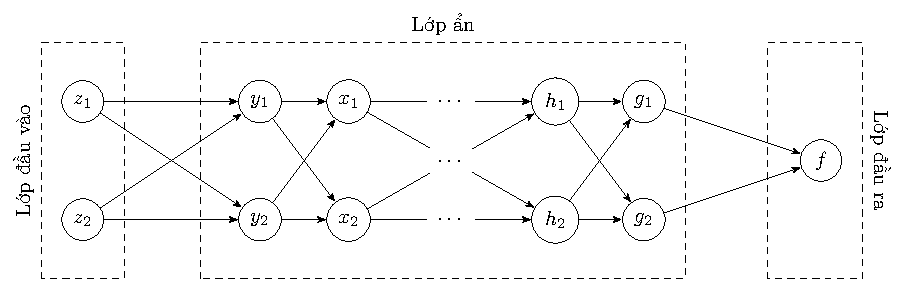
\includegraphics[width=0.8\textwidth]{tikz_image/complexity_graph.pdf}
    \caption{Mạng thần kinh với $n$ lớp, mỗi lớp có 2 nút}
    \label{figure:n-layer-2-node-nn}
\end{figure}
\begin{figure}[htb]
    \centering
    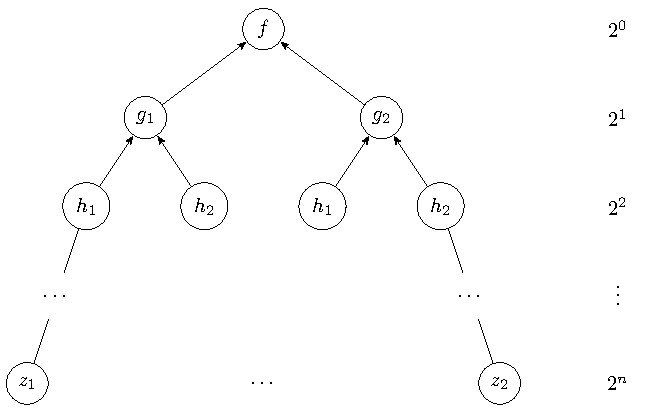
\includegraphics[width=0.5\textwidth]{tikz_image/complexity_tree.pdf}
    \caption{Đồ thị tính toán của mạng ở hình \ref{figure:n-layer-2-node-nn}}
    \label{figure:computational-graph-of-n-layer-2-node-nn}
\end{figure}

Nhìn đồ thị tính toán, để tìm công thức tổng quát của hàm $f$ dựa trên đầu vào $z_1,z_2$, ta phải khai triển các hàm lồng nhau. Ở tầng đầu tiên ta không có hàm lồng nhau nên số hàm lồng nhau phải khai triển là $2^0=1$, ở tầng thứ hai có một lớp lồng nhau là $f(g_1,g_2)$ nên số hàm phải khai triển là $2^1=2$, tương tự khi ta đi qua từng lớp đến đến lớp cuối cùng $n$, thì tổng số hàm lồng nhau mà ta phải khai triển là $2^n$. Độ phức tạp khi tính toán sẽ tăng theo cấp số nhân khi mà số lượng lớp tăng lên.

Để giải quyết vấn đề đầu tiên, nghĩa là không phải tính các hàm lồng nhau, người ta đưa ra giải pháp là áp dụng quy tắc xích (\textit{chain rule}) liên tục lặp đi lặp lại để tính đạo hàm ở từng lớp kế nhau (đạo hàm ở lớp $m$ đối với các nút ở lớp $m-1$), việc này làm giảm độ phức tạp vì chỉ phải tính đạo hàm trên một lớp duy nhất, không cần phải khai triển toàn bộ hàm. Bắt đầu tính đạo hàm ở lớp cuối cùng $n$, sau đó ta truyền giá trị đạo hàm xuống lớp kề nó (lớp $n-1$) để tính đạo hàm ở lớp này, rồi lặp lại quá trình này cho đến đầu đầu vào. Quá trình này gọi là lan truyền ngược, và việc tính toán theo cách số học (\textit{numerically}) cho từng lớp kế nhau sẽ dễ dàng hơn nhiều với việc tính toán kiểu đại số (\textit{algebraically}) trên toàn mạng rồi thay số vào.

Nhắc lại quy tắc xích
\begin{align}
    \dfrac{\partial f(g(x))}{\partial x} = \dfrac{\partial f(g(x))}{\partial g(x)}\cdot\dfrac{\partial g(x)}{\partial x}
\end{align}
\begin{figure}[htb]
    \centering
    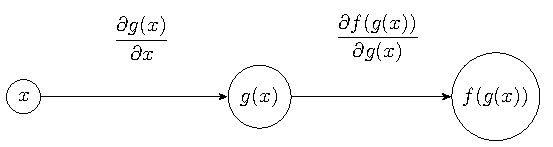
\includegraphics[width=0.5\textwidth]{tikz_image/chain_rule.pdf}
    \caption{Áp dụng quy tắc xích trong thần kinh đơn giản}
    \label{figure:chain-rule-nn}
\end{figure}
Đối với mạng thần kinh đơn giản (hình \ref{figure:chain-rule-nn}) với một nút đầu vào, một nút ẩn và một nút đầu ra, áp dụng quy tắc xích làm đơn giản hoá việc tính đạo hàm trên toàn mạng bằng việc tính đạo hàm trên từng cạnh rồi nhân với nhau. Đối với mạng thần kinh phức tạp hơn gồm nhiều lớp ẩn, mỗi lớp gồm nhiều nút, thì ta phải áp dụng quy tắc xích đa biến (\textit{multivariate chain rule})
\begin{align}
    \dfrac{\partial f(g_1(x),\dots,g_k(x))}{\partial x} = \sum^k_{i=1}\dfrac{\partial f(g_1(x),\dots,g_k(x))}{\partial g_i(x)}\cdot\dfrac{\partial g_i(x)}{\partial x}
\end{align}
Áp dụng quy tắc xích đa biến vào mạng (hình \ref{figure:multivariate-chain-rule-nn}), ta được
\begin{align}
    \label{equation:multivariate-chain-rule-nn}
    \dfrac{\partial o}{\partial x}=
    \dfrac{\partial f(g_1,g_2)}{\partial g_1}\cdot\dfrac{\partial g_1(h)}{\partial h}\cdot\dfrac{\partial h(x)}{\partial x}
    +\dfrac{\partial f(g_1,g_2)}{\partial g_2}\cdot\dfrac{\partial g_2(h)}{\partial h}\cdot\dfrac{\partial h(x)}{\partial x}
\end{align}
\begin{figure}[htb]
    \centering
    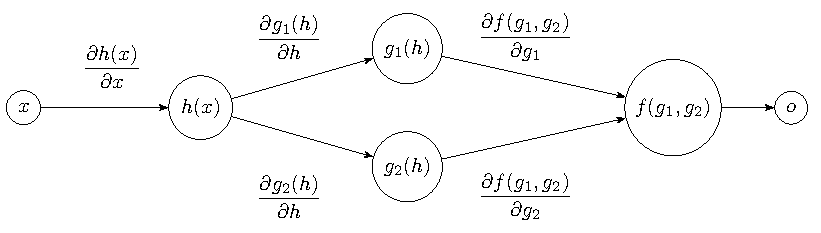
\includegraphics[width=0.8\textwidth]{tikz_image/multivariate_chain_rule.pdf}
    \caption{Áp dụng quy tắc xích đa biến trong mạng thần kinh phức tạp}
    \label{figure:multivariate-chain-rule-nn}
\end{figure}

Dựa vào quy tắc xích đa biến, Charu C. Aggarwal đã nêu ra bổ đề về tổng hợp của các cạnh (\textit{pathwise aggregation lemma}) \cite{Aggarwal2023-zk} như sau: gọi $y(i)$ là giá trị của nút $i$ trong mạng, gọi $z(i,j)=\partial y(j)/\partial y(i)$ là đạo hàm của cạnh $(i,j)$, gọi tập hợp các đường đi khác nhau xuất phát từ điểm $s$ và kết thúc ở điểm $t$ là $\mathcal{P}$, giá trị của đào hàm $\partial y(t)/\partial y(s)$ được tính bằng tích của các cạnh nối từ $s$ đến $t$, rồi lấy tổng theo các đường đi khác nhau dẫn từ $s$ đến $t$
\begin{align}
    \dfrac{\partial y(t)}{\partial y(s)}=\sum_{P\in\mathcal{P}}\ \prod_{(i,j)\in P}z(i,j)
    \label{equation:pathwise-aggregation-lemma}
\end{align}
Giải pháp này chỉ giải quyết được vấn đề đầu tiên mà không giải quyết được vấn đề thứ hai. Trong ví dụ hình \ref{figure:multivariate-chain-rule-nn}, có 2 con đường dẫn từ đầu vào đến đầu ra. Hai con đường này đều đi qua điểm $h(x)$, nên trong đạo hàm của hàm \ref{equation:multivariate-chain-rule-nn}, ta thấy có sự xuất hiện 2 lần của đạo hàm $\partial h(x)/\partial x$, nghĩa là nếu một cạnh $(i,j)$ xuất hiện trong $n$ đường đi ${P_1,\dots,P_n}\in\mathcal{P}$, thì ta phải tính đạo hàm của cạnh $(i,j)$ $n$ lần. Để giải quyết vấn đề tính trùng nhau này, người ta dùng phương pháp quy hoạch động (\textit{dynamic programming}) trong lý thuyết đồ thị (\textit{graph theory}).

Gọi $S(i,j)=\partial y(j)/\partial y(i)$, ta viết lại bổ đề \ref{equation:pathwise-aggregation-lemma} thành
\begin{align}
    S(s,t)=\sum_{P\in\mathcal{P}}\ \prod_{(i,j)\in P}z(i,j)
\end{align}
Chọn điểm $i$ bất kỳ trong mạng, gọi $j\in A(i)$ là tập hợp các điểm mà $i$ kết nối đến. Nếu tất cả giá trị của điểm $S(j,t)$ đã được tính, thì ta có hàm cập nhật $S(i,t)$ dựa trên các giá trị đã tính $S(j,t)$ là
\begin{align}
    S(i,t)=\sum_{j\in A(i)}z(i,j)S(j,t)
\end{align}
Với giá trị khởi tạo $S(t,t)=1$, mã giả của thuật toán quy hoạch động để tính $S(s,t)$ là
\begin{algorithmz}
    \caption{Mã giả tính $S(s,t)$ bằng quy hoạch động \cite{Aggarwal2023-zk}}
    \label{algorithm:dynamic-programming-node-to-node}
    \begin{algorithmic}[1]
        \State Khởi tạo $S(t,t)=1$
        \Repeat
        \State Chọn nút $i$ thoả tất cả giá trị $S(j,t)$ đã được tính, với $j\in A(i)$
        \State Cập nhật $S(i,t)\gets\sum_{j\in A(i)}z(i,j)S(j,t)$
        \Until tất cả các nút đã được tính
    \end{algorithmic}
\end{algorithmz}

Trong hầu hết các thuật toán học máy truyền thống, người ta chỉ cần tìm lời giải một lần duy nhất là một hàm $f$ dưới dạng rút gọn, sau đó chỉ cần thay các điểm dữ liệu khác nhau là ta sẽ cập nhật được bộ tham số $\mathbf{w}$ dựa theo thuật toán xuống đồi. Đối với thuật toán lan truyền ngược, ta phải chạy lại thuật toán với mỗi điểm khác nhau. Điều này nghe như khối lượng công việc sẽ nhiều hơn so với các thuật toán truyền thống, nhưng nó đã được chứng minh là tốt hơn nhiều so với cách giải truyền thống khi mà số lượng lớp và nút ở mỗi lớp lớn.

Như đã nói ở trên, sau khi đã tính được đạo hàm của $\partial y(j)/\partial y(i)$, ta phải suy ra đạo hàm của $\partial L/\partial\mathbf{w}$. Nếu mạng thần kinh có $p$ nút đầu ra, thì các nút đầu ra sẽ là $t_1,t_2,\dots,t_p$, hàm mất mát bây giờ sẽ là $L(y(t_1),y(t_2),\dots,y(t_p))$. Gọi $w_{ji}$ là tham số cạnh giữa hai nút $j$ và $i$. Khi này đạo hàm riêng của hàm mất mát sẽ là
\begin{align}
    \dfrac{\partial L}{\partial w_{ji}} & =
    \dfrac{\partial L}{\partial y(i)}\cdot\dfrac{\partial y(i)}{\partial w_{ji}\label{equation:loss-to-weight}}                                                                                                          \\
                                        & =\left[\sum^p_{k=1}\dfrac{\partial L}{\partial y(t_k)}\cdot\dfrac{\partial y(t_k)}{\partial y(i)}\right]\dfrac{\partial y(i)}{\partial w_{ji}}\label{equation:loss-to-weight1}
\end{align}
Giá trị của $\partial y(i)/\partial w_{ji}$ ($j$ là điểm nối đến $i$) có thể được tính theo hình \ref{figure:single-layer-network}. Giá trị của $\partial y(t_k)/\partial y(i)$ được tính bằng thuật toán quy hoạch động bên trên. Giá trị của $\partial L/\partial y(t_k)$ được tính như các thuật toán học máy truyền thống vì $L=L(y(t_1),y(t_2),\dots,y(t_p))$. Nhưng thay vì dùng thuật toán \ref{algorithm:dynamic-programming-node-to-node} để tính từng phần của \ref{equation:loss-to-weight1}, ta có thể biến đổi thuật toán này để tính $\partial L/\partial y(i)$.

Chọn điểm $i$ bất kỳ trong mạng, gọi $j\in A(i)$ là tập hợp các điểm mà $i$ kết nối đến. Đặt $\triangle(i)=\partial L/\partial y(i)$, dựa vào \ref{equation:loss-to-weight1}, ta có thể tính $\triangle(i)$ dựa trên các giá trị đã tính $\triangle(j)$
\begin{align}
    \triangle(i)=\sum_{j\in A(i)}z(i,j)\triangle(j)
\end{align}
Khởi tạo đạo hàm mất mát với tất cả các nút đầu ra $\triangle(t_k)$, ta có
\begin{algorithmz}
    \caption{Mã giả tính $\partial L/\partial\mathbf{w}$ bằng quy hoạch động \cite{Aggarwal2023-zk}}
    \label{algorithm:dynamic-programming-loss-to-weight}
    \begin{algorithmic}[1]
        \State Khởi tạo $\triangle(t_k)=\dfrac{\partial L}{\partial y(t_k)}$ với mỗi $k\in\{1,\dots,p\}$
        \Repeat
        \State Chọn nút $i$ thoả tất cả giá trị $\triangle(j)$ đã được tính, với $j\in A(i)$
        \State Cập nhật $\triangle(i)\gets\sum_{j\in A(i)}z(i,j)\triangle(j)$
        \Until tất cả các nút đã được tính
        \ForEach {cạnh $(j,i)$ có hệ số $w_{ji}$}
        \State Tính $\dfrac{\partial L}{\partial w_{ji}}\gets\triangle(i)\cdot\dfrac{\partial y(i)}{\partial w_{ji}}$
        \EndFor
    \end{algorithmic}
\end{algorithmz}\\
Sau khi tính $\partial L/\partial\mathbf{w}$, ta có thể áp dụng thuật toán xuống đồi để tối ưu tham số $\mathbf{w}$
\begin{align}
    \mathbf{w}\leftarrow\mathbf{w}-\alpha\cdot\dfrac{\partial L}{\partial\mathbf{w}}
\end{align}

Thuật toán \ref{algorithm:dynamic-programming-loss-to-weight} chỉ có thể áp dụng trong mạng thần kinh nhân tạo không có hàm kích hoạt. Gọi $B(i)$ là các nút kết nối đến nút $i$, $A(i)$ là các nút mà $i$ kết nối đến. Giá trị của nút trước khi qua hàm kích hoạt là $a(i)$, sau khi qua hàm kich hoạt là $h(i)=\Phi_i=\Phi(a(i))$. Khai triển của nút $i$ sẽ là một hàm tuyến tính các nút nối đến nó $a(i)=\sum_{j\in B(i)}w_{ji}h(j)$. Khi sử dụng hàm kích hoạt, ta phải biến đổi thuật toán theo một trong hai cách sau:
\begin{enumerate}
    \item Cách đầu tiên là sử dụng giá trị sau khi kích hoạt (\textit{post-activation}). Nếu ta đặt giá trị của nút $i$ là $y(i)=h(i)=\Phi(a(i))$ (giá trị sau hàm kích hoạt), thì trong thuật toán \ref{algorithm:dynamic-programming-loss-to-weight}, ta phải chú ý
          \begin{itemize}
              \item Giá trị $z(i,j)_{j\in A(i)}=\dfrac{\partial y(j)}{\partial y(i)}$ thay đổi thành
                    \begin{align}
                        z(i,j)
                         & =\dfrac{\partial\Phi(a(j))}{\partial\Phi(a(i))}                                          \nonumber \\
                         & =\dfrac{\partial\Phi(a(j))}{\partial a(j)}\cdot\dfrac{\partial a(j)}{\partial\Phi(a(i))} \nonumber \\
                         & =\Phi'_j\cdot w_{ij}
                    \end{align}
                    nên $\triangle(i)\gets\sum_{j\in A(i)}\left[\Phi'_j\cdot w_{ij}\right]\triangle(j)$
              \item Thay đổi
                    \begin{align}
                        \left[\dfrac{\partial y(i)}{\partial w_{ji}}\right]_{j\in B(i)}=\dfrac{\partial\Phi(a(i))}{\partial w_{ji}}=\dfrac{\partial\Phi(a(i))}{\partial a(i)}\cdot\dfrac{\partial a(i)}{w_{ji}}=\Phi'_i\cdot\Phi_j
                    \end{align}
                    nên $\dfrac{\partial L}{\partial w_{ji}}\gets\triangle(i)\left[\Phi'_i\cdot\Phi_j\right]$
          \end{itemize}
    \item Cách thứ hai là sử dụng giá trị trước khi kích hoạt (\textit{pre-activation}). Nếu ta đặt giá trị của nút $i$ là $y(i)=a(i)$ (giá trị trước hàm kích hoạt), thì mỗi khi tính giá trị $a(i)$ từ $a(j),j\in B(i)$, ta phải dùng hàm kích hoạt lên các giá trị đầu vào này $y(i)=a(i)=\sum_{j\in B(i)}\Phi(a(j))$. Lưu ý, vì ta chọn cách biến đổi $y(i)=a(i)$ nên ở lớp ẩn đầu tiên ta sẽ không phải tính hàm kích hoạt, và ở lớp đầu ra ta phải dùng hàm kích hoạt lên lớp này rồi mới đưa kết quả vào hàm mất mát.
          \begin{itemize}
              \item Giá trị khởi tạo sẽ là
                    \begin{align}
                        \dfrac{\partial L}{\partial y(t_r)}
                         & =\dfrac{\partial L}{\partial a(t_r)}                                                        \nonumber \\
                         & =\dfrac{\partial L}{\partial\Phi(a(t_r))}\cdot\dfrac{\partial\Phi(a(t_r))}{\partial a(t_r)} \nonumber \\
                         & =L'(\Phi_{t_r})\cdot\Phi'_{t_r}
                    \end{align}
                    % nên $\
              \item Tương tự như trên, giá trị $z(i,j)_{j\in A(i)}$ thay đổi thành
                    \begin{align}
                        z(i,j)
                         & =\dfrac{\partial a(j)}{\partial a(i)}                                                    \nonumber \\
                         & =\dfrac{\partial a(j)}{\partial\Phi(a(i))}\cdot\dfrac{\partial\Phi(a(i))}{\partial a(i)} \nonumber \\
                         & =w_{ij}\cdot\Phi'_i
                    \end{align}
                    nên $\triangle(i)\gets\Phi'_i\sum_{j\in A(i)}w_{ij}\cdot\triangle(j)$
              \item Thay đổi
                    \begin{align}
                        \left[\dfrac{\partial y(i)}{\partial w_{ji}}\right]_{j\in B(i)}=\dfrac{\partial a(i)}{\partial w_{ji}}=\Phi_j
                    \end{align}
                    nên $\dfrac{\partial L}{\partial w_{ji}}\gets\triangle(i)\cdot\Phi_j$
          \end{itemize}
\end{enumerate}

Cả hai cách trên đều được dùng trong mạng thần kinh nhân tạo, nhưng cách sử dụng giá trị trước khi kích hoạt thường được dùng nhiều hơn. Một số đạo hàm của hàm kích hoạt $\Phi'$ ở hình \ref{figure:differential-activation-funtion}.
\begin{figure}[htbp]
    \centering
    \begin{subfigure}[b]{0.33\textwidth}
        \centering
        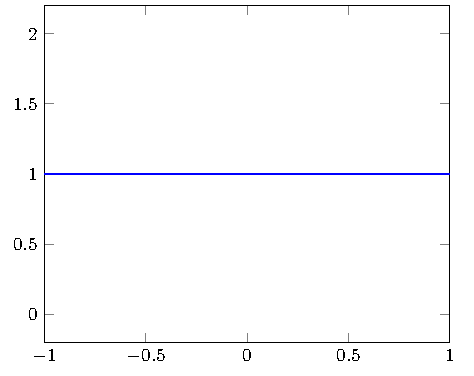
\includegraphics[width=\textwidth]{tikz_image/diff_identity.pdf}
        \caption{Hàm tuyến tính}
    \end{subfigure}%
    \begin{subfigure}[b]{0.33\textwidth}
        \centering
        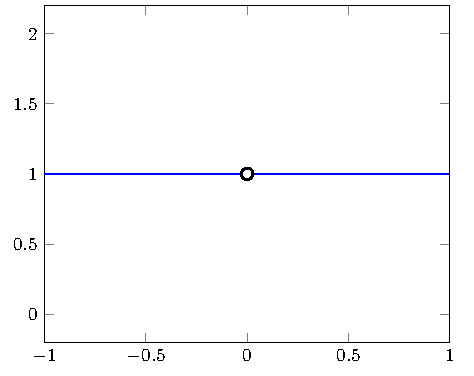
\includegraphics[width=\textwidth]{tikz_image/diff_sign.pdf}
        \caption{Hàm sign}
    \end{subfigure}%
    \begin{subfigure}[b]{0.33\textwidth}
        \centering
        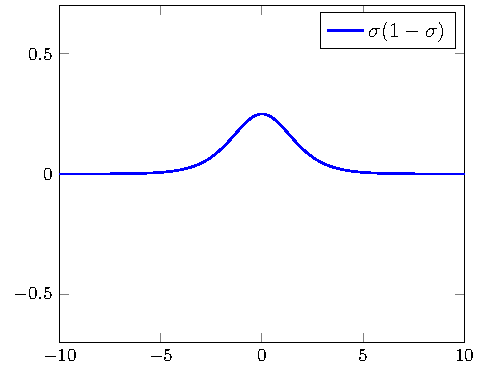
\includegraphics[width=\textwidth]{tikz_image/diff_sigmoid.pdf}
        \caption{Hàm sigmoid}
    \end{subfigure}\newline
    \begin{subfigure}[b]{0.33\textwidth}
        \centering
        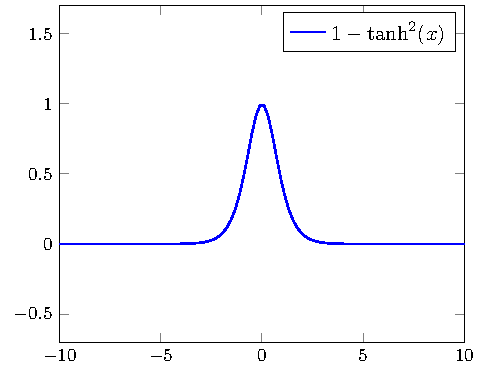
\includegraphics[width=\textwidth]{tikz_image/diff_tanh.pdf}
        \caption{Hàm tanh}
    \end{subfigure}%
    \begin{subfigure}[b]{0.33\textwidth}
        \centering
        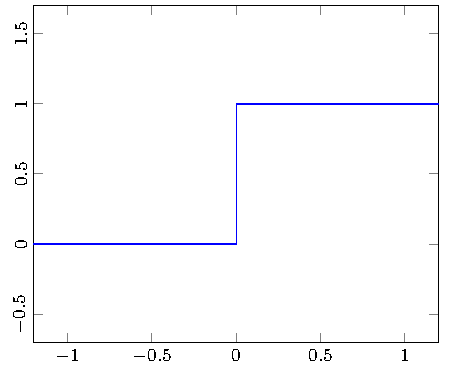
\includegraphics[width=\textwidth]{tikz_image/diff_relu.pdf}
        \caption{Hàm ReLu}
    \end{subfigure}%
    \begin{subfigure}[b]{0.33\textwidth}
        \centering
        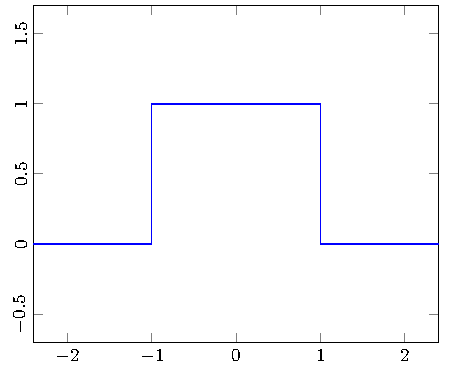
\includegraphics[width=\textwidth]{tikz_image/diff_hardtanh.pdf}
        \caption{Hàm hardtanh}
    \end{subfigure}%
    \caption{Đồ thị đạo hàm các hàm kích hoạt thông dụng}
    \label{figure:differential-activation-funtion}
\end{figure}

Đối với hàm kích hoạt softmax ở lớp đầu ra, ta không thể dùng thuật toán trên được mà phải thay đổi một chút ở lớp đầu ra khi đi qua hàm softmax. Gọi $o_1,\dots,o_p$ là giá trị xác suất của các biến đầu ra $t_1,\dots,t_p$, hàm softmax sẽ là
\begin{align}
    o_i=\dfrac{\exp(t_i)}{\sum_{j=1}^k\exp(t_j)}
\end{align}
Hàm softmax ở lớp đầu ra thường đi chung với hàm mất mát cross-entropy
\begin{align}
    L=-\sum_{i=1}^k y_i\log(o_i)
\end{align}
với $y_i$ là mã hoá one-hot của giá trị quan sát. Đạo hàm của hàm mất mát là
\begin{align}
    \label{equation:softmax-derivative}
    \dfrac{\partial L}{\partial t_i}
    =\sum_{j=1}^k\dfrac{\partial L}{\partial o_j}\cdot\dfrac{\partial o_j}{\partial t_i}
\end{align}
Với đạo hàm của hàm mất mát được tính theo mỗi đầu ra $o_j$
\begin{align}
    \dfrac{\partial L}{\partial o_j}=\dfrac{\partial[-y_j\log(o_j)]}{\partial o_j}=-\dfrac{y_j}{o_j}
\end{align}

Với hàm chỉ thị (\textit{indicator function}) $I(i,j)$, đạo hàm của giá trị sau và trước lớp softmax được tính bằng cách: \cite{webpage3}
\begin{align}
    \dfrac{\partial\log(o_j)}{\partial t_i}           & =\dfrac{1}{o_j}\cdot\dfrac{\partial o_j}{\partial t_i}                                                                                  \\
    \Leftrightarrow\dfrac{\partial o_j}{\partial t_i} & =o_j\cdot\dfrac{\partial\log(o_j)}{\partial t_i}
    =o_j\cdot\dfrac{\partial}{\partial t_i}\log\left[\dfrac{\exp(t_j)}{\sum_{l=1}^k\exp(t_l)}\right]                                                                                  \nonumber \\
                                                      & =o_j\cdot\left[\dfrac{\partial t_j}{\partial t_i}-\dfrac{\partial}{\partial t_i}\log\left[\sum_{l=1}^k\exp(t_l)\right]\right] \nonumber \\
                                                      & =o_j\cdot\left[\dfrac{\partial t_j}{\partial t_i}-\dfrac{\exp(t_i)}{\sum_{l=1}^k\exp(t_l)}\right]                             \nonumber \\
                                                      & =o_j\cdot(I(i,j)-o_i)
\end{align}
Thay vào phương trình \ref{equation:softmax-derivative}, ta có
\begin{align}
    \dfrac{\partial L}{\partial t_i}
     & =\sum_{j=1}^k-\dfrac{y_j}{o_j}\cdot o_j\cdot(I(i,j)-o_i) \nonumber \\
     & =o_i\sum_{j=1}^k y_j-\sum_{j=1}^k I(i,j)y_j              \nonumber \\
     & =o_i-y_i
\end{align}

Thuật toán \ref{algorithm:dynamic-programming-loss-to-weight} sau khi sửa đổi để sử dụng với hàm kích hoạt $\Phi$ là hoàn chỉnh để lập trình mạng thần kinh nhân tạo trên máy tính. Tuy nhiên thuật toán này không sử dụng các tính toán trên ma trận nên không thể tận dụng được sức mạnh phần cứng của GPU hay các thiết bị XLA. Vì thế ta cần thay đổi thuật toán về dạng ma trận (phương trình \ref{equation:matrix-form}) để tối ưu sức mạnh tính toán.

Ta quy ước đạo hàm đối với một vector sẽ được viết dưới dạng ma trận sắp xếp theo mẫu số (\textit{denominator layout}). Ví dụ ta có hai vector cột $\textbf{h}$ và $\textbf{x}$, ma trận của đạo hàm là
\begin{align}
    \left[\dfrac{\partial\mathbf{h}}{\partial\mathbf{x}}\right]_{ij}=\dfrac{\partial h_j}{\partial x_i}
\end{align}
Ma trận này chính là ma trận Jacobi chuyển vị $\left[\dfrac{\partial\mathbf{h}}{\partial\mathbf{x}}\right]=J(\mathbf{h},\mathbf{x})^\intercal$.

Nếu $\mathbf{o}=F_k(F_{k-1}(\dots F_1(\mathbf{x})))$, với đầu vô của hàm $F_i$ có chiều là $n_i$, đầu ra của hàm $F_i$ có chiều là $n_{i+1}$, thì quy tắc xích khi viết dưới dạng ma trận sắp xếp theo mẫu số sẽ là
\begin{align}
    \underbrace{\left[\dfrac{\partial\mathbf o}{\partial\mathbf x}\right]}_{n_1\times n_{k+1}}=
    \underbrace{\left[\dfrac{\partial\mathbf h_1}{\partial\mathbf x}\right]}_{n_1\times n_2}
    \underbrace{\left[\dfrac{\partial\mathbf h_2}{\partial\mathbf h_1}\right]}_{n_2\times n_3}\cdots
    \underbrace{\left[\dfrac{\partial\mathbf h_{k-1}}{\partial\mathbf h_{k-2}}\right]}_{n_{k-1}\times n_k}
    \underbrace{\left[\dfrac{\partial\mathbf h_k}{\partial\mathbf h_{k-1}}\right]}_{n_k\times n_{k+1}}
\end{align}
Quy tắc xích này có thứ tự đảo ngược so với quy tắc xích bình thường vì ta đang quy ước ma trận của đạo hàm sẽ dưới dạng sắp xếp theo mẫu số.

Mỗi nút trong mạng thần kinh nhân tạo sẽ được tính qua hai bước là bước tổng tuyến tính và bước sử dụng hàm kích hoạt, nên ta sẽ chia mỗi lớp trong mạng thành hai lớp riêng biệt, lớp đầu tiên là lớp tuyến tính (phương trình \ref{equation:matrix-form}), sau đó là lớp kích hoạt (hình \ref{figure:multi-layer-linear-activation-matrix}).
\begin{figure}[htb]
    \centering
    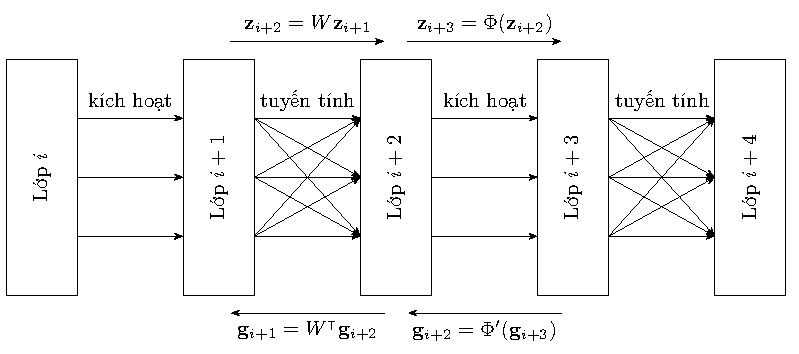
\includegraphics[width=0.8\textwidth]{tikz_image/multi_layer_linear_activation_matrix.pdf}
    \caption{Hai lớp tuyến tính và kích hoạt nằm xen kẽ nhau}
    \label{figure:multi-layer-linear-activation-matrix}
\end{figure}

Gọi $\mathbf z_i$ là vector giá trị của lớp $i$, $\mathbf g_i$ là vector đạo hàm $[\partial L/\partial\mathbf z_i]$, ta có
\begin{align}
     & \mathbf z_{i+1}=W\mathbf z_i                                                                      & \text{[Lan truyền xuôi ở lớp tuyến tính]} \\
     & \mathbf z_{i+1}=\Phi(\mathbf z_i)                                                                 & \text{[Lan truyền xuôi ở lớp kích hoạt]}  \\
     & \mathbf g_i=\left[\dfrac{\partial\mathbf z_{i+1}}{\partial\mathbf z_i}\right]\cdot\mathbf g_{i+1} & \text{[Lan truyền ngược]}                 % \left[\dfrac{\partial L}{\partial\mathbf z_i}\right]=\left[\dfrac{\partial\mathbf z_{i+1}}{\partial\mathbf z_i}\right]\left[\dfrac{\partial L}{\partial z_{i+1}}\right]
\end{align}

Một số hàm thường gặp trong mạng thần kinh khi lan truyền xuôi và lan truyền ngược (được tính dựa vào phương trình lan truyền ngược bên trên), với phép toán $\odot$ là tích Hadamard (\textit{Hadamard product} hay \textit{element-wise product}), vector $1s$ là \textbf 1.
\begin{table}[htbp]
    \centering
    \caption{Một số hàm thông dụng và lan truyền xuôi-ngược của nó \cite{Aggarwal2023-zk}}
    \label{table:derivative-forward-backward}
    \begin{threeparttable}
        \begin{tabularx}{\textwidth}{ c c C{1} C{1} }
            \toprule
            \textbf{Hàm}      & \textbf{Kiểu hàm} & \textbf{Lan truyền xuôi}                              & \textbf{Lan truyền ngược}                                                           \\\midrule
            linear            & nhiều-nhiều       & $\mathbf z_{i+1}=W\mathbf z_i$                        & \tnote{1}$\mathbf g_i=W^\intercal\mathbf g_{i+1}$                                   \\\midrule
            sigmoid           & một-một           & $\mathbf z_{i+1}=\text{sigmoid}(\mathbf z_i)$         & $\mathbf g_i=\mathbf g_{i+1}\odot\mathbf z_{i+1}\odot(\mathbf 1-\mathbf z_{i+1})$   \\\midrule
            tanh              & một-một           & $\mathbf z_{i+1}=\tanh(\mathbf z_i)$                  & $\mathbf g_i=\mathbf g_{i+1}\odot(\mathbf 1 - \mathbf z_{i+1}\odot\mathbf z_{i+1})$ \\\midrule
            ReLU              & một-một           & $\mathbf z_{i+1}=\mathbf z_i\odot I\ (z_i^{(r)}>0)$   & $\mathbf g_i=\mathbf g_{i+1}\odot I\ (z_i^{(r)}>0)$                                 \\\midrule
            max               & nhiều-một         & $r=z_i^{(k)}\geq z_i^{(j)},\forall j\in\{1,\dots,p\}$ & \tnote{2}$\mathbf g_i=[0,\dots,z_i^{(k)},\dots,0]^\intercal$                        \\\midrule
            $f(\cdot)$ bất kỳ & bất kỳ            & $\mathbf z_{i+1}=f(\mathbf z_i)$                      & \tnote{3}$\mathbf g_i=J^\intercal\mathbf g_{i+1}$                                   \\
            \bottomrule
        \end{tabularx}
        \begin{tablenotes}
            \item[1] Do quy ước ma trận sắp xếp theo mẫu nên ta phải chuyển vị kết quả đạo hàm.
            \item[2] Hàm $\max$ thực sự không có đạo hàm, vì sự thay đổi nhỏ của các giá trị $z_i^{(j)}$ khác giá trị tối đa $z_i^{(k)}$ không hề ảnh hưởng đến kết quả. Chỉ có duy nhất giá trị tối đa $z_i^{(k)}$ là ảnh hưởng đến đầu ra cho nên ta cho tất cả giá trị $g_i^{(j)}(j\neq k)=0$.
            \item[3] Với $J$ là ma trận Jacobi $J_{kr}=\dfrac{\partial f_k(\mathbf z_i)}{\partial z_i^{(r)}}$
        \end{tablenotes}
    \end{threeparttable}
\end{table}

Sau khi lan truyền xuôi để tính toàn bộ $\mathbf z_i$, lan truyền ngược để tính toàn bộ $\mathbf g_i$, ta phải tính đạo hàm của hàm mất mát trên trọng số cạnh. Gọi $p$ là nút ở lớp $i-1$, giá trị nút này sẽ là $z_{i-1\ p}$. Gọi $q$ là nút ở lớp $i$, giá trị nút này sẽ là $z_{iq}$. Ta có
\begin{align}
    \dfrac{\partial L}{\partial w_{pq}}=\dfrac{\partial L}{\partial z_{iq}}\cdot\dfrac{\partial z_{iq}}{\partial w_{pq}}=\underbrace{g_{iq}\cdot z_{i-1\ p}}_{1\times 1}
\end{align}
Với quy ước ma trận sắp xếp theo mẫu số, ma trận đạo hàm của hàm mất mát $L$ đối với ma trận tham số cạnh $W$ được tính bằng tích ngoài (\textit{outer product}) \cite{Aggarwal2023-zk}
\begin{align}
    M=\mathbf g_i\cdot\mathbf  z_{i-1}^\intercal
\end{align}


\subsubsection{Các vấn đề gặp phải khi huấn luyện mạng thần kinh}
Mạng thần kinh có hàng triệu tham số $w_{ij}$ trong đó một số cạnh có giá trị đạo hàm $\partial L/\partial w_{ij}$ rất lớn so với các thành phần khác, dẫn đến thuật toán xuống đồi cập nhật một phần bộ tham số quá lệch so với phần còn lại. Điều đó tương đương với việc một số lớp ảnh hưởng trực tiếp đến lớp đầu ra, còn một số lớp thì hầu như chẳng có ảnh hưởng. Điều này xuất hiện chủ yếu là do giá trị đạo hàm được tính toán bằng quy tắc xích và nhân liên tục với nhau. Xét một mạng thần kinh với $m$ lớp, để đơn giản ta xem mỗi lớp chỉ có duy nhất 1 nút, giá trị của nút ở lớp ẩn thứ $t+1$ là
\begin{align}
    h_{t+1}=\Phi(w_{t+1}h_t)
\end{align}

Đạo hàm từ nút $t+1$ đối với nút $t$ là
\begin{align}
    \dfrac{\partial h_{t+1}}{\partial h_t}=w_{t+1}\cdot\Phi'(w_{t+1}h_t)
\end{align}

Đạo hàm từ hàm mất mát đối với nút $t$ sẽ có dạng
\begin{align}
    \dfrac{\partial L}{\partial h_t}=\dfrac{\partial L}{\partial h_{t+1}}\cdot\dfrac{\partial h_{t+1}}{\partial h_t}=w_{t+1}\cdot\Phi'(w_{t+1}h_t)\cdot\dfrac{\partial L}{\partial h_{t+1}}
\end{align}

Nếu ta khởi tạo các giá trị $w_k$ dựa theo phân phối chuẩn, thì giá trị trung bình của $w=1$. Nếu ta chọn hàm kích hoạt là hàm sigmoid, đạo hàm của nó sẽ là $\Phi'=\sigma(1-\sigma)$, giá trị của hàm sigmoid nằm trong khoảng $(0,1)$ nên dạo hàm này có giá trị lớn nhất là $\Phi'=0.25<1$ khi $\sigma=0.5$. Nghĩa là đạo hàm của lớp sau luôn bé hơn hoặc bằng $0.25$ giá trị của lớp trước nó. Nếu ta đi ngược $r$ lớp thì đạo hàm lớp $t-r$ sẽ bé hơn hoặc bằng $0.25^r$ giá trị lớp $t$. Do đó khi ta cập nhật bộ tham số bằng thuật toán lan truyền ngược thì tham số cạnh $w$ của các lớp trước sẽ được điều chỉnh ít hơn nhiều so với các lớp sau, vấn đề này gọi là độ dốc biến mất (\textit{vanishing gradient problem}). Nếu ta chọn một hàm kích hoạt cho ra giá trị $\Phi'>1$ thì trường hợp ngược lại sẽ xảy ra: tham số cạnh $w$ của các lớp trước sẽ được điều chỉnh nhiều hơn so với các lớp sau, vấn đề này gọi là độ dốc bùng nổ (\textit{exploding gradient problem}).

Tổng quát trong mạng thần kinh có nhiều lớp, mỗi lớp có nhiều nút. Gọi $A$ là ma trận đạo hàm của lan truyền ngược $\mathbf g_i = A\mathbf g_{i+1}$ đối với lớp kích hoạt. Vì là ma trận đạo hàm của lớp kích hoạt nên nó thường là ma chận chéo (bảng \ref{table:derivative-forward-backward}) nên ta có thể chéo hoá ma trận này thành $A=PDP^{-1}$. Quy tắc xích trong lan truyền ngược là tích liên tục của $A$, tương đương với $A^t=PD^tP^{-1}$. Nghĩa là độ dốc biến mất sẽ xảy ra khi các giá trị riêng $\lambda$ của $A$ nhỏ hơn $1$, ngược lại sẽ xảy ra độ dốc bùng nổ. \cite{Aggarwal2023}

Có nhiều cách để hạn chế vấn đề này, cách đơn giản là ta phải chọn hàm kích hoạt sao cho đạo hàm của nó luôn ở lân cận $1$, và đạo hàm này phải cho cả giá trị $1^-$ và $1^+$. Ví dụ ta chọn các hàm kích hoạt từng phần như ReLU sẽ giá trị đạo hàm là $0$ hoặc $1$, nghĩa là giờ đây độ dốc bùng nổ và độ dốc biến mất sẽ ít xảy ra hơn. Nhưng đối với các giá trị âm, nó sẽ không cập nhật lại trọng số vì đạo hàm của nó bằng $0$ tại các điểm này. Điều đó dẫn đến trọng số nối với nút này không được học nữa, đầu ra của nó luôn bằng $0$ nên nút này không có ý nghĩa, vấn đề này gọi là nút chết (\textit{dead neurons}). Một cách để khắc phục vấn đề này là dùng hàm ReLU bị rò rỉ (\textit{leaky ReLU}). Trong thực tế thì không tồn tại hàm kích hoạt nào để giải quyết triệt để vấn đề này mà ta chỉ có thể làm giảm đi ảnh hưởng của nó lên mạng.
